\documentclass[a4paper,11pt]{jsbook}


% 数式
\usepackage{amsmath,amsfonts}
\usepackage{bm}
% 画像
\usepackage[dvipdfmx]{graphicx}
\usepackage[dvipdfmx]{color}

\begin{document}

\title{Splatoon}
\author{さとうあずき}
\date{\today}
\maketitle
\tableofcontents

\part{初めに}
\chapter{準備}
\section{コントローラーの操作}
ZRでメインウェポンで攻撃ができる。Lスティックでキャラクターを移動できる。
\begin{figure}
  \begin{center}
    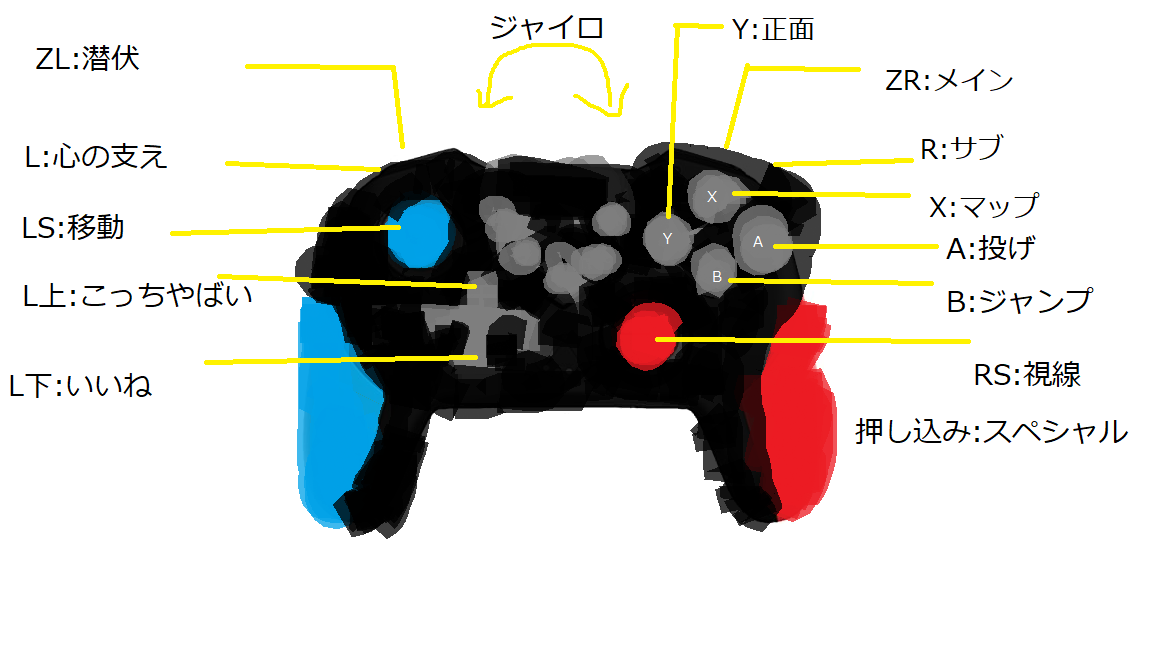
\includegraphics[width=10cm]{resoource/Controller_button.png}
  \end{center}
\end{figure}

試合画面
上に味方と敵のイカマークがある。敵味方の存命がわかる。
右上にスペシャルゲージがある。たまったら、Rスティック押し込みでスペシャルウェポンが使える。
画面中心にレティクルがある。この中に敵を入れてメインウェポンで狙える。ZRでメインウェポンで倒せる。
\begin{figure}
  \begin{center}
    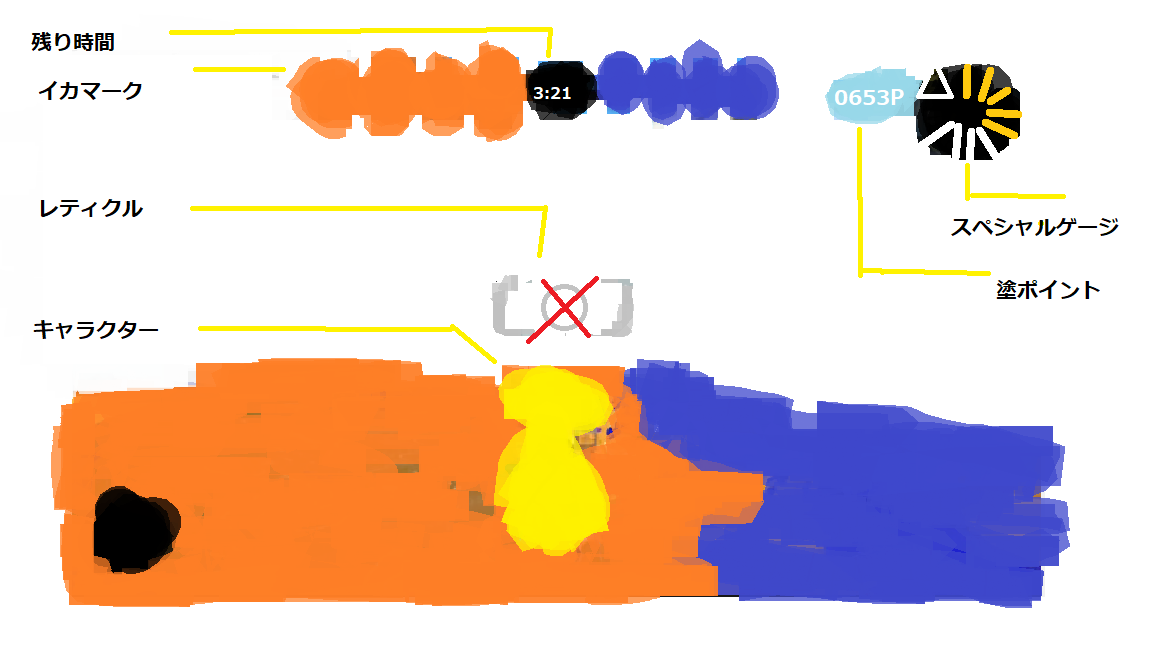
\includegraphics[width=10cm]{resoource/gamescreenframe.png}
  \end{center}
\end{figure}
\section{敵の倒し方}



\section{ゲームが目指しているところ}
人は目が覚めたらご飯を食べ、トイレに行き、将来に向けてあくせくと働き、そして寝る。
最適化された生活の中には喜怒哀楽もなく、ただ平然と人生を消費していき、死ぬ。
最適化された生活から脱却するような無駄な行為である。
しかし、人生において無駄な行為こそ、人生を謳歌するための唯一の手段である。
人生においてゲームは必要ない。だからこそゲームの中での一喜一憂は我々の生活を豊かにし、そして生まれた意味になる。

\section{Splatoon3とは}
Splatoon3は2022年9月8日に任天堂から発売開始され、発売3日間で国内販売本数345万本を記録した大人気ゲームソフトである。
このゲームはイカやタコが4対4のチームを組み、インクを垂らしながら陣地を奪ったりルールに基づいてポイントを稼いだりして勝敗を決める、新感覚のシューティングゲームである。
老若男女問わず楽しめるもので初心者からプロもプレイし、このゲームを通して世界中のプレイヤーはゲームのランキングを競いあっている。

\section{Splatoonへの憤り}
Splatoonは大変面白いゲームであり、世界中から愛されている。
素晴らしいプレイがあれば喜び、強い敵に打ち負かされて悲しみ、このゲームを通して我々は充実した時間を過ごすことができるだろう。
しかし、Splatoonをこよなく愛するプレイヤーの中にはどうやらただただストレスをうけ、さらにそのプレイヤーの罵声や怒号によって周りの人間を不愉快にさせ、何のためにゲームをやっているのかわからなくなっている人がいるようだ。
私はそんな人たちが少しでも充実したゲーム人生を過ごしてもらうと、筆を執ることにした。

\chapter{準備}
\section{ゲームを楽しむ}


\section{勝負に勝つ}


\section{試合に勝つ}





\part{試合を優位に進める}
\chapter{大局的人数有利}
\section{通信障害}
\section{イカマーク}
\section{マッチルールオブジェクト}
マッチルールオブジェクトを味方と考える。→三角関係

\chapter{局所的人数有利}
\section{三角関係}
自分と相手と何か
味方
ルール関与オブジェクト
自分の残像



\section{戦線}
敵と味方が打ち合っている境界線
\begin{figure}
  \begin{center}
    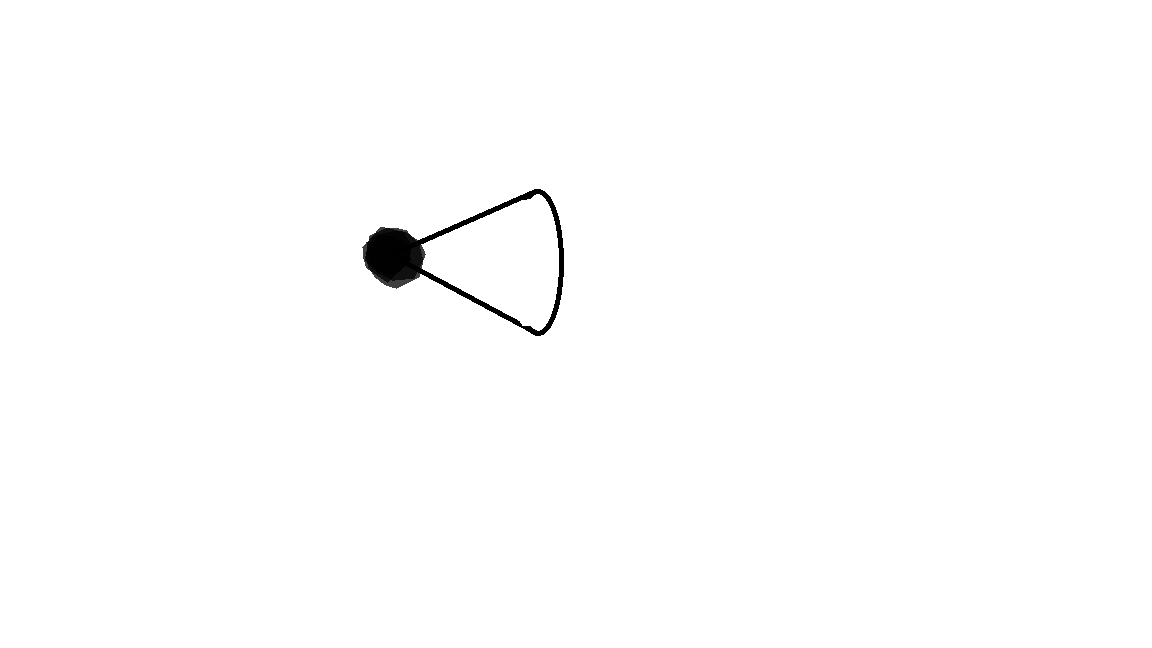
\includegraphics[width=10cm]{resoource/player.png}
  \end{center}
\end{figure}

\section{前線}
戦線にヘルプに入れる位置で自陣のリスボーンに一番近い位置

\chapter{地形有利}
\section{高所}
相手の位置がわかる、自分の位置は相手はわからない

\section{オブジェクト}
\chapter{チーム構成有利}
\section{スペシャルウェポン有利}
打開
射程
\section{サブウェポン有利}
打開
射程
\section{メインウェポン有利}
打開
射程
\section{ギア有利}
打開
射程

\part{勝負を優位に進める}
\chapter{メインウェポン}
\section{射程と索敵}
\section{射程とキル}
\chapter{サブウェポン}
\section{索敵}
\chapter{スペシャルウェポン}
\chapter{イカ状態とヒト状態}
\section{当たり判定}
ヒト状態とイカ状態
右打ち
\section{インク回復}
\section{移動速度}
\section{インク潜伏}
\chapter{マップ}
\chapter{キャラクター移動}
\section{風神雷神}
\chapter{スーパージャンプ}
\chapter{ジャンプ}
\chapter{やられたとカモンとナイス}
\chapter{カメラリセット}

\part{ガチマッチで勝つ}
\chapter{ガチエリア}
\section{カウントを進める}
マッチルールオブジェクトと前線、戦線
マッチルールオブジェクトはエリアになり、エリアはステージ中心に存在する。
オブジェクト付近に敵を近づけさせないために、前線はステージ中心より敵陣側
前線と敵陣リスポーンの間に戦線が発生する

\section{カウントを奪う}
マッチルールオブジェクトと前線、戦線
マッチルールオブジェクトはエリアになり、エリアはステージ中心に存在する。
オブジェクト付近に近づくために、前線がステージ中心にある
戦線と自陣リスポーンの間に前線が発生する


\chapter{ガチヤグラ}
\chapter{ガチホコ}
\chapter{ガチアサリ}

\part{終わりに}
\chapter{謝辞}

\appendix
\chapter{A}



\begin{thebibliography}{2}

\bibitem{K.miyuki}K.miyuki (private communication)
\end{thebibliography}

\thispagestyle{empty}
\vspace*{\stretch{1}}
\begin{flushright}
\begin{minipage}{0.5\hsize}
\begin{description}
  \item{著者:}さとうとーま
  \item{挿絵:}さとうとーま
  \item{発行:}\date{\today}
  % \item{印刷:}POPLS (\verb|http://www.inv.co.jp/~popls/|)
\end{description}
\end{minipage}
\end{flushright}

\end{document}











